
%\documentclass[gray,trans]{beamer} % com o mod transpar�ncia
%\documentclass[gray]{beamer}
\documentclass[trans,note]{beamer}
\setbeamertemplate{footline}[frame number] % Mostra o n�mero de frames e n�o o de slides.

\usetheme{Frankfurt}
%\usetheme{Madrid}

%\usetheme{Marburg} % Template ideial para SBMF
%\usetheme{CambridgeUS}
 %\usetheme{Boadilla}
\usetheme{default}


%\usecolortheme{structure} 
%\usebeamercolor{structure}

% \usefonttheme[onlylarge]{structurebold}
% \usefonttheme{default}
% \setbeamerfont*{frametitle}{size=\normalsize,series=\bfseries}
 % \setbeamertemplate{navigation symbols}{}

% \usepackage[latin1]{inputenc} 
% \usepackage[brazil]{babel}
\usepackage[english]{babel}
\usepackage[latin1]{inputenc}

\usepackage{graphicx,url}
\usepackage{fancyhdr}

\usepackage{tikz}
\usetikzlibrary{arrows}
 \tikzstyle{block}=[draw opacity=0.3,line width=1.0cm]

% Class options include: notes, notesonly, handout, trans,
% hidesubsections, shadesubsections,
% inrow, blue, red, grey, brown

% Theme for beamer presentation.
%\usepackage{beamerthemeclassic}
% \usepackage{beamerthemebars}
% \usepackage{beamerthemesplit}
% \usepackage{beamerthemetree}
% \usepackage{beamerthemelined}



\title{Formal Modelling of \\ a Microcontroller Instruction Set in B}

\pgfdeclareimage[height=0.35cm]{b2asm}{figures/b2asm.pdf}
\logo{\pgfuseimage{b2asm}}


%\subtitle{Qualifica��o de Mestrado} % Enter your title betweencurlybraces
\author{Val�rio Medeiros Jr, David D�harbe}
\institute{Federal University of Rio Grande do Norte} % Enter your institute name between curly braces
\date{20 August 2009} % Enter the date or \today between curly braces

\begin{document}

%% Keywords for the B method

\newcommand{\MACHINE}{\ensuremath{\textbf{MACHINE }}}

%\newcommand{\MACHINE}{\operatorname{\textbf{MACHINE }}} % COMANDO ORIGINAL
\newcommand{\REFINEMENT}{\operatorname{\mathbf{REFINEMENT }}}
\newcommand{\IMPLEMENTATION}{\ensuremath{\textbf{IMPLEMENTATION }}}
\newcommand{\REFINES}{\ensuremath{\textbf{REFINES }}}
\newcommand{\SEES}{\ensuremath{\textbf{SEES }}}
\newcommand{\INCLUDES}{\ensuremath{\textbf{INCLUDES }}}
\newcommand{\IMPORTS}{\ensuremath{\textbf{IMPORTS }}}
\newcommand{\SETS}{\ensuremath{\textbf{SETS }}}
\newcommand{\CONSTANTS}{\ensuremath{\textbf{CONSTANTS }}}
\newcommand{\PROPERTIES}{\ensuremath{\textbf{PROPERTIES }}}
\newcommand{\CONCRETE}{\ensuremath{\textbf{CONCRETE }}}
\newcommand{\VARIABLES}{\ensuremath{\textbf{VARIABLES }}}
\newcommand{\ASSERTIONS}{\ensuremath{\textbf{ASSERTIONS }}}
\newcommand{\CONCRETEVARIABLES}{\ensuremath{\textbf{CONCRETE\_VARIABLES }}}
\newcommand{\DEFINITIONS}{\ensuremath{\textbf{DEFINITIONS }}}
\newcommand{\VAR}{\ensuremath{\textbf{VAR }}}
\newcommand{\IN}{\ensuremath{\textbf{IN }}}
\newcommand{\INVARIANT}{\ensuremath{\textbf{INVARIANT }}}
\newcommand{\INITIALISATION}{\ensuremath{\textbf{INITIALISATION }}}
\newcommand{\OPERATIONS}{\ensuremath{\textbf{OPERATIONS }}}
\newcommand{\BEGIN}{\ensuremath{\textbf{BEGIN }}}
\newcommand{\END}{\ensuremath{\textbf{END }}}
\newcommand{\PRE}{\ensuremath{\textbf{PRE }}}
\newcommand{\IF}{\ensuremath{\textbf{IF }}}
\newcommand{\THEN}{\ensuremath{\textbf{THEN }}}
\newcommand{\ELSE}{\ensuremath{\textbf{ELSE }}}
\newcommand{\ELSIF}{\ensuremath{\textbf{ELSIF }}}
\newcommand{\ANY}{\ensuremath{\textbf{ANY }}}
\newcommand{\WHERE}{\ensuremath{\textbf{WHERE }}}
\newcommand{\CASE}{\ensuremath{\textbf{CASE }}}
\newcommand{\OF}{\ensuremath{\textbf{OF }}}
\newcommand{\EITHER}{\ensuremath{\textbf{EITHER }}}
\newcommand{\AND}{\ensuremath{\textbf{AND }}}
\newcommand{\OR}{\ensuremath{\textbf{OR }}}
\newcommand{\NOT}{\ensuremath{\textbf{NOT }}}
\newcommand{\WHILE}{\ensuremath{\textbf{WHILE }}}
\newcommand{\DO}{\ensuremath{\textbf{DO }}}
\newcommand{\VARIANT}{\ensuremath{\textbf{VARIANT }}}
\newcommand{\FALSE}{\ensuremath{\textbf{FALSE }}}
\newcommand{\TRUE}{\ensuremath{\textbf{TRUE }}}

%% Commonly used math entities
\newcommand{\pow}{\ensuremath{\textbb{P }}}
\newcommand{\nat}{\ensuremath{\textbb{N }}}
\newcommand{\pfun}{\ensuremath{\rightarrow\mkern-22mu+}}
\newcommand{\fset}{\ensuremath{\textbb{F }}}
\newcommand{\dom}{\ensuremath{\mbox{dom}}}
\newcommand{\ran}{\ensuremath{\mbox{ran}}}
\newcommand{\natone}{\ensuremath{\textbb{N}_1}}
\newcommand{\integer}{\ensuremath{\textbb{Z }}}
%\newcommand{\fun}{\ensuremath{\rightarrow}}
\newcommand{\domr}{\ensuremath{\triangleleft}}
\newcommand{\seq}{\ensuremath{\textbf{seq1 }}}
\newcommand{\ovr}{\ensuremath{\oplus}}
\newcommand{\BOOL}{\ensuremath{\textbf{BOOL }}}
\newcommand{\pred}{\ensuremath{\textbf{pred }}}
\newcommand{\Bsucc}{\ensuremath{\textbf{succ }}}


\include{SymbolsB_AtelierB}

\beamertemplatefootpagenumber % Mostra o n�mero de p�ginas

% Creates title page of slide show using above information
\begin{frame}
   \titlepage  
  \begin{center} 
  Project: B2ASM\\
  Available at http://code.google.com/p/b2asm\\
  \includegraphics[width=.14\textwidth]{figures/ufrn.png} \ \ \ \ \ \ \ \ \ \ \ \ \ \ \ \ \ \ \ 
  \includegraphics[width=.14\textwidth]{figures/anp.png}  \ \ \ \ \ \ \ \ \ \ \ \ \ \ \ \ \ \ \
   \includegraphics[width=.12\textwidth]{figures/dimap.png}
  \end{center}
  
\end{frame}
\note{Initial Slide} % Add notes to yourself that will be displayed when
  % typeset with the notes or notesonly class options


%\section [Agenda]{Agenda}


% Creates table of contents slide incorporating
% all \section and \subsection commands
 \begin{frame}
  \frametitle{Summary}
  \tableofcontents
 \end{frame} 

% Mostra um slide com destaque a atual se��o, em cada mudan�a de se��o
% \AtBeginSection[]
% {
% \begin{frame}
% \frametitle{Summary}
% \tableofcontents[currentsection]
% \end{frame}
% }

  
\section{Introduction}


\begin{frame}
\frametitle{Initial Overview}

\begin{itemize}[<+->]
  \item The B method supports the construction of safety systems
  \begin{itemize}
    \item Until the implementation model
    \item But part of this translation is not guaranteed by formal means\\
    \begin{center}
       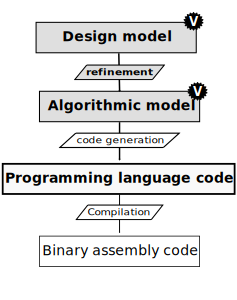
\includegraphics[height=.5\textheight]{figures/b-method-actual_new.pdf}
    \end{center}
       \begin{itemize} \item   \small{The transformation process can introduce small bugs}
       \end{itemize}
  \end{itemize}
\end{itemize}
   

	\note{ ................... }
	
\end{frame}



\begin{frame}
\frametitle{Extended Overview}  

\begin{itemize}[<+->]
    \item We proposed [Dantas, 2008]  a approach to extend the formal verification
    \item One key of this approach is the formal model of the instruction set  of execution platform % of such assembly languages
      \\ \begin{center} 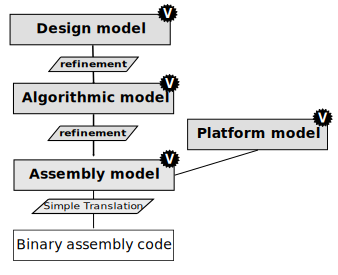
\includegraphics[height=.5\textheight]{figures/b-method-ideal_new.pdf} \end{center}
  

\end{itemize}
% TO-DO Ajustar a figura

	\note{ ................... }
\end{frame}


\begin{frame}
\frametitle{Modelling Assembly Instruction Set in B}  

\begin{itemize}[<+->]
  \item We developed libraries of hardware models%.The modelling is builded using some  developed libraries
  \item The libraries have common concepts that can be used to others platforms of 8 or 16 bits
  \item Utilities of this formal model:
  \begin{itemize}
    \item Documentation
    \item Simulation
    \item The formal verification until the assembly level
    \item A possible support to verify the Z80 design

  \end{itemize}
\end{itemize}

	\note{ ................... }
\end{frame}


% 
% \begin{frame}
% \frametitle{Objective}  
% 
% \begin{itemize}[<+->]
%   \item The main actual objective is represent the assembly instruction set
%     \begin{itemize}
%     \item The aspects no-functional are not represented: logic circuits, pipeline, data bus, \ldots 
%   \end{itemize}
%   \item Moreover there are many efficient ways to verify hardware
% 
% \end{itemize}
% % 
% 
% 	\note{ ................... }
% \end{frame}
% 



%  % * Explain the cover of B Method 
%  % The solution is a framework proposed a paper [Dantas, 2009]
%  % The component key to this aproach is the formal model
%  % Then this paper gave u
% 
  \section{B Method}

\begin{frame}
\hypertarget{metodoB}{}
  \frametitle{B Method} 
  \begin{itemize}
    \item B method for software development is a formal method based on
	    \begin{itemize}
	    \item  B Abstract Machine Notation (AMN)
	    \item  First order logic, integer arithmetic and set theory
	    \end{itemize}
    \item It is similar to the Z notation
%     \begin{itemize} \item But it has also the substitution calculus and the
%     refinement calculus
%     \end{itemize}   
    \item Supports:
    \begin{itemize}
	    \item Modularization
	    \item Advanced techniques for proof development: user pass,
	    parallelization, etc.
	    \item Refinements proved up to basic constructs of programming language  
	    \item Code generator to programming language
	    \item \ldots
    \end{itemize}   
  \end{itemize}
\end{frame}
    
    
%     
% \begin{frame}
% \frametitle{B Method- Simple example}
% \begin{figure}
%   % \begin{small}
%   $$
%   \begin{array}{lcl}
%     \begin{array}[t]{l}
%       \MACHINE \\ \quad  \mathit{micro} \\
%       \SEES \\ \quad \mathit{TYPES}, \mathit{ALU} \\
%       \INCLUDES \\  \quad \mathit{MEMORY} \\
%       \VARIABLES \\ \quad    \mathit{pc}  \\
%       \INVARIANT \\ \quad \mathit{pc} \in \mathit{INSTRUCTION} 
%     \end{array}
%     & \hspace*{0cm} &
%     \begin{array}[t]{l}
%       \INITIALISATION  \mathit{pc} := 0 \\
%       \OPERATIONS\\
%       \mathit{JMP} \mathit{( jump )} = \\
%       \quad \PRE \mathit{jump} \in \mathit{INSTRUCTION}\\ 
%       \quad \THEN \mathit{pc} := \mathit{jump}\\  
%       \quad \END \\
%       \END
%     \end{array}
%   \end{array}
%   $$
% \caption{A very basic B machine.}
% \label{fig:maqB}
% \end{figure}
% \end{frame}
%  %  Basear-se nas notas escritas 
% 
  \section{Modelling the Instruction Set in B}
\begin{frame}
  \frametitle{Modelling  Microcontrollers}  

  \begin{itemize}[<+->]
  \item Relations 
  \begin{itemize}
  	\item States of platform  $\Leftrightarrow$ States of modell
		\begin{itemize}
		\item Registers and Memory $\Leftrightarrow$  Variables of model
		\end{itemize}
	\item Assembly Instructions $\Leftrightarrow$ B operations
        \begin{itemize}
        \item Changes of states of platform $\Leftrightarrow$ B substitutions
        \end{itemize}
  \end{itemize}
    
 \end{itemize}
\end{frame}


\begin{frame}
 \frametitle{Structure of Projects B}
 \begin{center}\includegraphics[width=1.\textwidth]{figures/diagramaEstrutural_vertical.png}
 \end{center}

 \end{frame}

 

 
\begin{frame}
 \frametitle{Project Hardware Library}

  	  	\begin{itemize}
 
  	  		\item Definition of \textit{Bit}
  			{\small
 			$
 			\begin{array}{l}
 			\mathit{BIT} = 0..1 \\
 			\end{array}
 			$
 			}
 
 			\item The function $\mathit{bit\_not}$ is a unary function:
			{\small
			$
			\begin{array}{l}
			\mathit{bit\_not}  \in  \mathit{BIT}  \fun  \mathit{BIT}  \land \\
			\forall (\mathit{bb}).(\mathit{bb} \in \mathit{BIT} \implies \mathit{bit\_not}(\mathit{bb}) = 1-\mathit{bb})\\
			\end{array}
			$
			}

			\item Some utils lemmas to development proofs

			{\small
			$
			\begin{array}{l}
			\mathit{bit\_not}(0) = 1; 	\mathit{bit\_not}(1) = 0; \\
			\forall (\mathit{bb}).(\mathit{bb} \in \mathit{BIT} \implies \mathit{bit\_not}(\mathit{bit\_not}(\mathit{bb})) = \mathit{bb});
			\end{array}
			$
			}
			\item The conjuction is a binary function defined as:
			{\small
			$
			\begin{array}{l}
			\mathit{bit\_and} \in \mathit{BIT} \times \mathit{BIT} \fun \mathit{BIT} \land \\
			\forall (\mathit{b1}, \mathit{b2}).(\mathit{b1}  \in \mathit{BIT}  \land \mathit{b2} \in \mathit{BIT} \implies \\
			\quad ((\mathit{bit\_and}(\mathit{b1}, \mathit{b2}) = 1) \iff (\mathit{b1} =1)  \land  (\mathit{b2} = 1))) \land \\
			 bit\_and(0,0) = 0	\land bit\_and(0,1) = 0	\land\\
			 bit\_and(1,0) = 0	\land bit\_and(1,1) = 1 \\
			\end{array}
			$
			}


  		\end{itemize}


\end{frame}


 
 
\begin{frame}
 \frametitle{Projeto \textit{Hardware Library}}

 	\begin{itemize}
 	  		\item The module \textit{BIT\_DEFINITION} has:

 	  		\begin{itemize}
 	  		\item Definiions of 	$\mathit{bit\_or},\mathit{bit\_xor}$ and
 	  		$bool\_to\_bit$.
 	  		\item Lemmas to associativity and commutativity of functions.
           \end{itemize}

			\item  The module \textit{BIT\_VECTOR\_DEFINITION} has

           \begin{itemize}
	 	  		\item Definition of bit vectors:
				{\small
				$
				\begin{array}{l}
				\mathit{BIT\_VECTOR} = \seq (\mathit{BIT}) % Implementa��o antiga, mas vale
				\end{array}
				$
				}
	 	  		\item Definition of functions:
	 	  		 {\small
				$
				\begin{array}{l}
				\mathit{bv\_size} \in \mathit{BIT\_VECTOR} \fun \nat_1 \land \\
				\mathit{bv\_size} = \lambda bv \bullet (bv \in \mathit{BIT\_VECTOR} \mid \mathbf{size}(bv))
				\end{array}
				$
				}
				\item It has others functions: \textit{bv\_catenate}, \textit{bv\_sub},
				\textit{bv\_not}, \textit{bv\_and}, \textit{bv\_or}, \textit{bv\_xor},
				\textit{bv\_set}, \textit{bv\_clear} e \ldots
			\begin{itemize}
	                  \item This functions using the definitions of  \textit{BIT\_DEFINITION}
	              	\end{itemize}
           \end{itemize}

           \item The module \textit{BIT\_VECTOR\_ARITHMETICS} define basics arithmetic functions
           \item The module \textit{BYTE} e \textit{BV16\_DEFINITION} define specialized functions to bit vectors of size 8 and 16
 	\end{itemize}


\end{frame}



\begin{frame}
 \frametitle{Types Library Project}
	  	\begin{itemize}
	        \item Define the common types and functions on platforms of 8 and 16 bits
	        \item For example:
	        \begin{itemize}
	          \item Function: \hspace*{0.0in}\it uchar\_schar  $\in$  \it UCHAR  $\fun$  \it SCHAR
	%  		  \hspace*{0.0in}\it uchar\_schar\rm = $\lambda$ \rm (\it v1\rm )\rm .\rm (\it v1 $\in$ \it UCHAR
	%  			$\land$  \it v1 $\leq$ \it SCHAR\_MAX $\mid$  \it v1\rm )  $\land$\\
	%  			\hspace*{0.0in}\it uchar\_schar\rm = $\lambda$ \rm (\it v1\rm )\rm .\rm (\it v1 $\in$ \it UCHAR
	%  			$\land$   $\neg$ \rm (\it v1 $\leq$ \it SCHAR\_MAX\rm )  $\mid$  \it v1\rm -\it UCHAR\_MAX \rm + \rm 1
	%  			\rm )
	
	
	          \item Lemma: $\forall(x).( x \in UCHAR \Rightarrow uchar\_byte(byte\_uchar(x)) = x)$
	        \end{itemize}
	      \end{itemize}
	
	\begin{table}[h]
	\begin{center}
	{\scriptsize
	\begin{tabular}{|c|c|c|c|c|c|c|}
	\hline
	 $Nome$&$\mathit{UCHAR}$&$\mathit{SCHAR}$&$\mathit{USHORTINT}$&$\mathit{SSHORTINT}$&$\mathit{BYTE}$&$\mathit{BV16}$\\
	 \hline $Faixa$&0..255&-128..127&0..65.535&-32.768..32.767&--&--\\ \hline
	 $Tamanho$ & 1 byte & 1 byte & 2 bytes & 2 bytes &  1 bytes & 2 bytes \\ \hline
	\end{tabular}
	}
	\end{center}
	\caption{Description of integer data types}
	\label{tab:types}
	\end{table}
\end{frame}

 
\begin{frame}
 \frametitle{Platform project(Z80)}
  \begin{itemize}
    \item Z80 is a microcontroller  of 8 bits with addressing of 16 bits
    \item Supports:
    \begin{itemize}
      \item 158 instructions (included all of 8080 microcontroller )
      \item Several addressing modes and interruption types
      \item 256 input and output ports (8 bits)
      \item Some operations with 16 bits
    \end{itemize}


      \item Header of modelling B
  \end{itemize}

	 {\scriptsize
	 \begin{sloppypar}
	\hspace*{1.0in}\bf MACHINE\\
	\hspace*{1.15in}\it Z80\\
	\hspace*{1.0in}\bf INCLUDES\\
	\hspace*{1.10in}\it MEMORY\\
	\hspace*{1.0in}\bf SEES\\
	\hspace*{1.10in}\it ALU, \it BIT\_DEFINITION, \it BIT\_VECTOR\_DEFINITION,\\
	\hspace*{1.10in}\it BYTE\_DEFINITION, \it BV16\_DEFINITION,\\
	\hspace*{1.10in}\it UCHAR\_DEFINITION, \it SCHAR\_DEFINITION,\\
	\hspace*{1.10in}\it SSHORT\_DEFINITION ,\it USHORT\_DEFINITION\\
	\end{sloppypar}
	}

\end{frame}

\begin{frame}
\frametitle{Modelling Registers, input/output ports and instructions from Z80}

 \begin{itemize}
   \item The invariant:

	{\scriptsize
	\begin{sloppypar}
	%\bf INVARIANT\\
	\hspace*{0.10in}\it rgs8  $\in$  \it id\_reg\_8  $\fun$  \it BYTE  $\land$ pc  $\in$  \it INSTRUCTION
	$\land$\\
	\hspace*{0.10in}\it  sp  $\in$  \it BV16  $\land$  \it ix  $\in$  \it BV16  $\land$  \it iy  $\in$  \it
	BV16  $\land$\\
	\hspace*{0.10in}\it i\_  $\in$  \it BYTE  $\land$  \it r\_ $\in$  \it BYTE  $\land$ iff1  $\in$  \it BIT
	$\land$ \it iff2  $\in$  \it BIT  $\land$ \\
	\hspace*{0.10in}\it im \rm $\in$ \rm (\it BIT $\times$ \it BIT\rm )  $\land$ \it i\_o\_ports  $\in$
	\it BYTE $\fun$  \it BYTE\\
	\end{sloppypar}
	}
	\item A simple instruction
	{\scriptsize
	\begin{sloppypar}
	\hspace*{0.10in}\bf LD\_n\_A \rm ( \it nn \rm ) \rm =\\
	\hspace*{0.20in}\bf PRE \it nn $\in$ \it USHORT\hspace*{0.15in}\\ %$\land$  \it nn $\in$\it DATA\_R\_ADR
	\hspace*{0.20in}\bf THEN\\
	\hspace*{0.20in}\bf updateAddressMem \rm ( \it ushort\_to\_bv16 \rm ( \it nn \rm ) \rm , \it rgs8 \rm ( \it a0 \rm )
	\rm )  $\para$\\
	\hspace*{0.20in}\it pc \rm := \it instruction\_next \rm ( \it pc \rm )  $\para$  \it r\_ \rm := \it
	update\_refresh\_reg\rm (\it r\_\rm )\\
	\hspace*{0.10in}\bf END\rm
	\end{sloppypar}

	}

	\end{itemize}
% \end{itemize}
% 	\begin{center}
% 	{\small
% 	$$
% 	\begin{array}{l}
% 	\mathit{BTFSS} (\mathit{ff}, \mathit{bb}) =\\
% 	\quad \PRE \mathit{ff} : \mathit{REGISTER} \land  \mathit{bb} : \mathit{BYTE\_INDEX} \\
% 	\quad \THEN \\
% 	\quad \quad	\IF \mathit{bitget}(\mathit{mem}(\mathit{ff}), \mathit{bb}) = 1 \THEN\\
% 	\quad\quad\quad	   \mathit{pc} :=\mathit{instruction\_next}(\mathit{instruction\_next}(\mathit{pc}))\\
% 	\quad\quad	\ELSE\\
% 	\quad\quad\quad	  \mathit{pc} := \mathit{instruction\_next}(\mathit{pc})\\
% 	\quad\quad	\END\\
% 	\quad \END
% 	\end{array}
% 	$$
% 	}\\
% 	Instru��o de controle do \textit{PIC16C432}
%
% 	\end{center}

\end{frame}

% 
%  \include{content/4_Description}
% 
  \section{Prove Process}

\begin{frame}
\frametitle{Prove Process of Projects}

\begin{itemize}
   \item Statistics:\\
    \begin{center}{\footnotesize
  	 \begin{tabular}{|c|c|c|c|}
		\hline
		 \textsl{Projects} &  \textsl{POs}	& \textsl{POs WD} &	\textsl{Total}\\
		\hline
		\textit{Power} & 	21 &	4 &	25\\
		\hline
		\textit{Types Library} &	22 &	68 &	90\\
		\hline
		\textit{Hardware Library} &	108 &	324 &	432\\
		\hline
		\textit{Z80} &	631	 & 2470 & 	3101\\
		\hline
		   &    &  & 		\textbf{3648}\\
		\hline
	 \end{tabular}
   }
	\end{center}

   \item  Approximately 25\% are not solved automatically
	\item  Approximately 18 days are needed to make almost all the proofs using a monolithic computer
		\begin{itemize}
			\item But You can reduce this time if you use several computer to prove
		\end{itemize}
	\item  Sometimes was needed  replay the proofs when were needed news fixes
\end{itemize}

\end{frame}


\begin{frame}
\frametitle{A example of user pass}

\begin{itemize}
   \item Specialized:
   \item \ldots
   \item Generally:
\end{itemize}

\end{frame}




%  % Example proof commands  
%  
%  \include{content/6_Related_works}
% 
   \section{Conclusions}





 \begin{frame}
 \frametitle{Considerations about the Work}
    
 \begin{itemize}
   \item It be able to: \ \ \ \ \ \ \ \ \ \ \ \ \ \ \ \ \ \ \ \ \ \ \ \ \ \ \ \ \ \ \ 
    \includegraphics[width=.2\textwidth]{figures/processador_generico.jpg}
 	\begin{itemize} 
 	  \item Identify  errors on the official reference
 	  \item Help assembly programmers
 	  \item Formal verification until assembly language 
     \end{itemize} 
     \item Future work is the verified development of a petroleum production test system\\ 
     \begin{center}   
 	   \includegraphics[height=.25\textheight]{figures/dutos.png}
	 \end{center}%\ \ \ \ \ \ \ \ \ \ 
     %   \includegraphics[height=.25\textheight]{figures/trem_bala2.png}
     
 \end{itemize} 
  	
 \end{frame}


\begin{frame}
  \frametitle{Sugestions/Doubts/Critics }
  	\begin{center}
    {\huge ?}\\
    \includegraphics[width=.5\textwidth]{figures/rodin.png}\\
    \large{ If you prefer, you can send an e-mail to 
    %\textcolor{blue!70!black}{\textit{valerio}}@ppgsc.ufrn.br or
    \textcolor{blue!70!black}{\textit{valerio.jr}}@gmail.com \\
    Project available at http://code.google.com/p/b2asm
    }
	\end{center}
    
\end{frame}
% 

  
   



\end{document}